% !TEX TS-program = pdflatex
% !TEX encoding = UTF-8 Unicode

% This is a simple template for a LaTeX document using the "article" class.
% See "book", "report", "letter" for other types of document.

\documentclass[11pt,twoside]{report} % use larger type; default would be 10pt

\linespread{1}
\renewcommand*\rmdefault{ptm}

\usepackage[utf8]{inputenc} % set input encoding (not needed with XeLaTeX)

%%% Examples of Article customizations
% These packages are optional, depending whether you want the features they provide.
% See the LaTeX Companion or other references for full information.

%%% PAGE DIMENSIONS
\usepackage{geometry} % to change the page dimensions
\geometry{a4paper} % or letterpaper (US) or a5paper or....
\geometry{
	margin=2.5cm,
} % for example, change the margins to 2 inches all round
% \geometry{landscape} % set up the page for landscape
%   read geometry.pdf for detailed page layout information

\usepackage{graphicx} % support the \includegraphics command and options

% \usepackage[parfill]{parskip} % Activate to begin paragraphs with an empty line rather than an indent

%%% PACKAGES
\usepackage{url}
\usepackage{booktabs} % for much better looking tables
\usepackage{array} % for better arrays (eg matrices) in maths
\usepackage{paralist} % very flexible & customisable lists (eg. enumerate/itemize, etc.)
\usepackage{verbatim} % adds environment for commenting out blocks of text & for better verbatim
\usepackage{subfig} % make it possible to include more than one captioned figure/table in a single float
\usepackage[final]{pdfpages}
% These packages are all incorporated in the memoir class to one degree or another...

%%% HEADERS & FOOTERS
\usepackage{fancyhdr} % This should be set AFTER setting up the page geometry
\pagestyle{fancy} % options: empty , plain , fancy
\renewcommand{\headrulewidth}{0pt} % customise the layout...
\lhead{\small Teaching Quantum Mechanics Using qCraft}\chead{}\rhead{\small Micha van den Enk, s1004654}
\lfoot[\small \today]{\small \thepage}
\cfoot{}
\rfoot[\small \thepage]{\small \today}

%%% SECTION TITLE APPEARANCE
\usepackage{sectsty}
\allsectionsfont{\sffamily\mdseries\upshape} % (See the fntguide.pdf for font help)
% (This matches ConTeXt defaults)

%%% RULE

\newcommand{\HRule}{\rule{\linewidth}{0.5mm}}

%%% BIBLIOGRAPHY

\usepackage{apacite}                           %bibliography in apa-style

%%% ToC (table of contents) APPEARANCE
\usepackage[nottoc,notlof,notlot]{tocbibind} % Put the bibliography in the ToC
\usepackage[titles,subfigure]{tocloft} % Alter the style of the Table of Contents
\renewcommand{\cftsecfont}{\rmfamily\mdseries\upshape}
\renewcommand{\cftsecpagefont}{\rmfamily\mdseries\upshape} % No bold!

\setcounter{secnumdepth}{-2}

%%% TABLES

\renewcommand{\arraystretch}{1.2}

\usepackage{afterpage}

\newcommand\blankpage{%
    \null
    \thispagestyle{empty}%
    \newpage}

%%% END Article customizations

%%% The "real" document content comes below...

\begin{document}

\begin{titlepage}

\begin{center}


% Upper part of the page

\includegraphics[width=1\textwidth]{./logo}\\[1cm]    

\textsc{\Large Bachelor Thesis}\\[0.5cm]
\textsc{\Large {[}201000166{]}}\\[0.5cm]


% Title
\HRule \\[0.4cm]
{ \huge \bfseries Teaching Quantum Mechanics Using qCraft}\\[0.4cm]

\HRule \\[1.5cm]

% Author and supervisor
\begin{minipage}{0.4\textwidth}
\begin{flushleft} \large
\emph{Author:}\\
Micha \textsc{van den Enk} \\
{[}s1004654{]} \\
\end{flushleft}
\end{minipage}
\begin{minipage}{0.4\textwidth}
\begin{flushright} \large
\emph{Supervisors:} \\
Dr. H. H. \textsc{Leemkuil} \\
Second \textsc{supervisor} \\
\end{flushright}
\end{minipage}

\vfill

% Bottom of the page
{\large \today}

\end{center}

\end{titlepage}

\afterpage{\blankpage}

\setcounter{tocdepth}{1}
\tableofcontents
\thispagestyle{fancy}
\newpage

\section{Preface}

%%% ANALYSIS

\subsection{The Generic Model}

\begin{figure}[h]
\centering
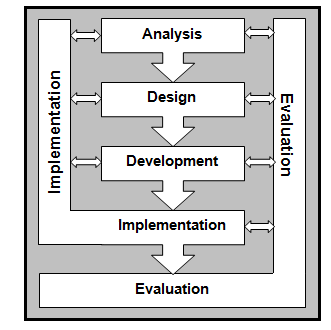
\includegraphics[width=0.7\textwidth]{genericmodel}
\caption{\footnotesize The generic model by \protect\citeA{genericmodel}\label{fig:genericmodel}}
\end{figure}

\subsection{Topics mentioned in literature}

The first logical question which should be asked would be the question which topics exist within the domain of introductory quantum mechanics, because only then we can delve into the question how these topics could or should be thought to novice learners. This exploration would have to start there where the students already familiar with. This is the Rutherford-Bohr Model of the Atom, also known as the Bohr Model, which presents a description of a hydrogen atom (see figure~\ref{fig:bohrmodel}). Students in upper secondary education should at least be familiar with this model, especially those with a technical profile. This gives way to introduce the students to the concept of elementary particles, which are the particles which exhibit quantum behaviour. The Bohr-model is also often referred to in the studied literature \cite{dori, mckagan, muller, papaphotis1, papaphotis2}.

\begin{figure}[h!]
\centering
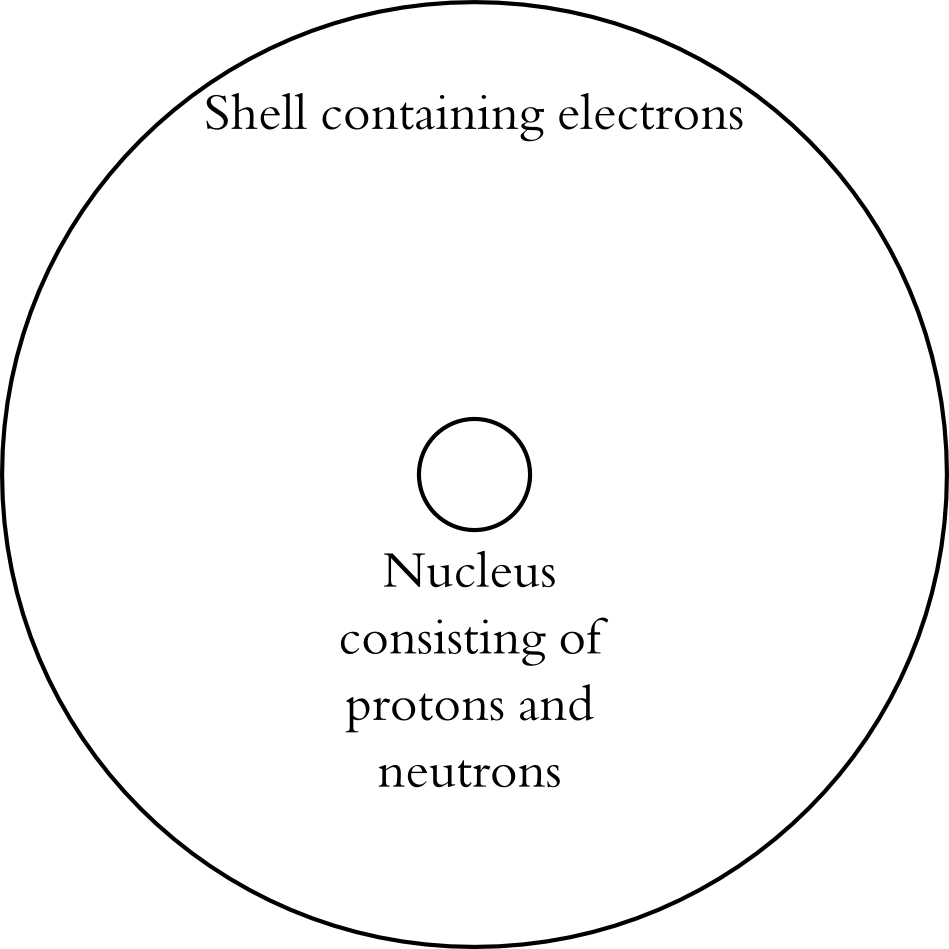
\includegraphics[width=0.5\textwidth]{bohrmodel}
\caption{The Rutherford-Borh Model of the Atom}
\label{fig:bohrmodel}
\end{figure}

The first logical question which should be asked would be the question which topics exist within the domain of introductory quantum mechanics, because only then we can delve into the question how these topics could or should be thought to novice learners. This exploration would have to start with a topic the students are already familiar with. Such a topic is the Rutherford-Bohr Model of the Atom, also known as the Bohr Model, which presents a description of a hydrogen atom (see figure~\ref{fig:bohrmodel}). Students in upper secondary education should at least be familiar with this model, especially those with a technical profile. This gives way to introduce the students to the concept of elementary particles, which are the particles which exhibit quantum behaviour. The Bohr-model is also often referred to in the studied literature \cite{dori, mckagan, muller, papaphotis1, papaphotis2}.

\begin{figure}[h!]
\centering
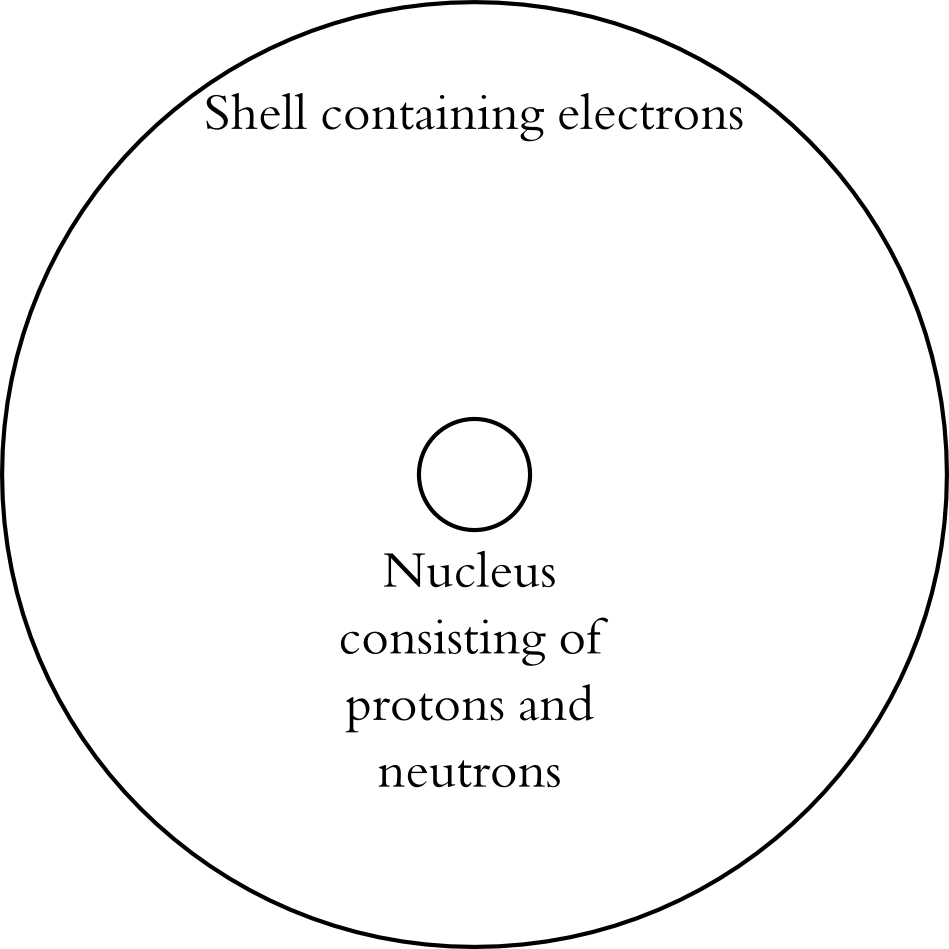
\includegraphics[width=0.5\textwidth]{bohrmodel}
\caption{The Rutherford-Borh Model of the Atom}
\label{fig:bohrmodel}
\end{figure}

Some of the studies \cite{erduran, hubber, muller, thacker} then describe properties of specific elementary particles, mostly of electrons or photons. Often used properties are the photoelectric effect or the polarisation of light \cite{henriksen, mckagan, muller}. These properties could give more meaning to what the elementary particles are and do. Another benefit would be that these properties are used in the various experiments conducted within the field of quantum mechanics.

The double-slit experiment is the most famous of these experiments, and also the most studied tool for educational purposes \cite{asikainen, henriksen, hobson, levrini, mckagan, muller, papaphotis1,singh2, thacker}. A reason why this experiment is famous is because it was the first experiment in history to demonstrate phenomena of quantum mechanics. The experiment entails shooting elementary particles through two narrow slits in a wall, projecting them on a large wall behind these two slits. When the two slits are separated very little, a interference pattern emerges. This is a result expected when the elementary particles would not be particles but waves. However, if the particles are observed and information is available through which slit each particle traversed, a diffraction pattern emerges, which would be the behaviour of particles. The most apparent phenomena demonstrated by this experiment is the wave-particle duality of elementary particles, which then could give way to mathematical descriptions of quantum mechanics like the Schrödinger equation. The Centraal Eindexamen of 2015 also already contained this experiment \cite{eindexamen2015}, so educational resources for teaching this experiment already exist.

For understanding the double-split experiment, the concept of superposition is vital. Superposition means that when a particle is not observed, it is in all possible states at the same time. In the case of the double-slit experiment, superposition means that the particle goes through both slits at the same time. It then interferes with itself because of the probability function of where the particle ends up. However, when the particle is observed through which slit it travels, the information through which slit the particle travels is known and forces the probability function of the particle to collapse to either the left or the right slit. Because of this, it behaves like a particle and a diffraction pattern emerges. A video which demonstrates the double-slit experiment can be seen on \url{https://upload.wikimedia.org/wikipedia/commons/transcoded/e/e4/Wave-particle_duality.ogv/Wave-particle_duality.ogv.480p.webm}. The double-slit experiment can provide the learner with an explanation of the observer dependency of the elementary particles. However, only \citeA{muller} mentions this concept in his study, and it also does not appear in the Centraal Eindexamen of 2016 \cite{eindexamen2016}.

The concept of superposition also has different cases. There are other properties of elementary particles which can be in superposition, for example the polarity of photons. Upon measurement, the polarisation value of a photon particle collapses to a certain value, but before this collapse it has all the different polarities at the same time. This gives way to the concept of entanglement, mentioned in some studies \cite{henriksen, hobson, kuttner}. Entanglement is a phenomenon which occurs between elementary particles, and it has as effect that the collapse of the different particles are interdependent of each other. This entanglement has two forms: boson entanglement and fermion entanglement. When the two particles are bosons, they always collapse to the same state on observation, and when the two particles are fermions, they always collapse to each others opposite state.

Since the discovery of the phenomena occurring within quantum mechanics, scientists have debated fiercely about how to interpret these phenomena \cite{barnes}. Roughly speaking, the scientists could be divided intro two camps: the camp of the realists and the camp of the ontologists. The realists thought that there has to be something underneath quantum mechanics which could explain the strange phenomena of superposition and entanglement, whereas the ontologists thought that the phenomena of quantum mechanics stand on its own. The phenomena of entanglement played a huge role in this debate. The realists first thought that they could use entanglement to prove that there is a reality underneath quantum mechanics, but it eventually led mostly to evidence towards the camp of ontologists. One example of this is Bell's inequalities \cite{kuttner, muller}, which is beyond the scope of this literature study to explain.

\citeA{henriksen} writes that there are three main differences between classical mechanics and quantum mechanics. The first difference is the fact that classical mechanics are deterministic and that quantum mechanics are probabilistic, also brought up by \citeA{levrini} and by \citeA{papaphotis1}. Classical mechanics rely heavily on deterministic causal effects, which can ultimately be explained. This is very apparent in systems of force, where everything moves according to certain laws, take for example the three Newtonian laws. Quantum mechanics however relies heavily on probabilistic models, where certain properties of certain elementary particles collapse to certain values according to probability functions.

A second difference between classical mechanics and quantum mechanics mentioned by \citeA{henriksen} is the locality of classical mechanics and the non-locality of quantum mechanics, also mentioned by \citeA{hobson}. On the scale of classical mechanics, it is possible to determine the exact position of an object, at least it is possible to do this on a significant scale. On a very small scale however, on the scale of quantum mechanics, the exact position of an object  cannot be determined. There is an inherent uncertainty about the position of an object, which is very small and insignificant on the scale of classical mechanics, but quite significant on the scale of elementary particles. This is also true for the momentum of an elementary particle, which can be translated to the speed of an elementary particle. This uncertainty can be demonstrated by the uncertainty principle of Heisenberg \cite{henriksen, muller, velentzas}, which has as implications that neither the location nor the momentum of an elementary particle can be exactly known and that the more certain the location of an elementary particle is known, the less certain the momentum of an elementary particle can be known and vice versa.

Finally, \citeA{henriksen} mentions that classical mechanics are continuous and that quantum mechanics are discrete. This is because of the Planck length, which is the shortest measurable length. In classical mechanics, this length is very insignificant, and because of that the world looks continuous. A fully continuous world would mean that there is no tiniest unit, but that it is always possible to “go smaller”. For example, if one had a plank of wood, it could be divided in half infinitesimally. However, on a quantum scale, this is not possible, because it is not possible to have something smaller than the Planck length.

Because of the inherent difficulty with quantum mechanics, some scientists have posited thought experiments, which allows the learner to make a mental model about the different concepts of quantum mechanics. The most famous thought experiment is that of Schrödingers cat \cite{muller, velentzas}, where the life of a cat depends on the collapse of an elementary particle. When the cat is then observed, the state of the elementary is observed indirectly, which causes it to collapse and either kill the cat or let the cat live. This teaches the student about observer dependency, the way observations are linked to the random collapse of an elementary particle. Another thought experiment mentioned in the studied literature is the EPR paradox \cite{kuttner, muller, velentzas}, which can be used to teach the student about how entanglement is related to deep questions about the nature of quantum mechanics. This thought experiment however is related to the EPR experiment, which lies beyond the scope of this study to explain.

Finally, there are some studies which recommend certain mathematical approaches to quantum mechanics, namely the Schrödingers equation \cite{muller, singh2}, the Hermitian operator \cite{singh2}, the aforementioned Bell's inequalities \cite{kuttner, muller}, the eigenvalue equation \cite{muller} and the DeBroglie energy levels \cite{dori, gianino, mckagan}. However, these mathematical approaches rely on a thorough conceptual understanding of quantum mechanics and are therefore not relevant to this study.

The topics relevant to teaching quantum mechanics can be summed up as the Rutherford-Bohr model of the Atom and elementary particles, the double-slit experiment, superposition, entanglement, the debate between realists and ontologists, the differences with classical mechanics, thought experiment and the mathematical side of quantum mechanics.

\chapter{Analyses}
\thispagestyle{fancy}

The first step of the Generic Model by \citeA{genericmodel} (see figure~\ref{fig:genericmodel} on page~\pageref{fig:genericmodel}) is Analysis. \citeA{smithragan} give an elaborated description of how to perform these analyses for instructional design. They distinguish three different kinds of analysis: analyzing the learner context, analyzing the learner and analyzing the learning task. The analysis of the learning context can provide the instructional needs and a description of the different factors influencing the instruction. The purpose of the learner analysis is the characterization of the end user of the instruction, which is in this case the middle school students. In the task analysis the test specifications are written, with which the content of the instruction can be established.These three analyses are executed in the following three chapters.

% Context Analysis

\section{Context Analysis}

A learning task always takes place in a certain learning context. In this case this is the middle school. It entails not only the place, but also the temporal and social environment \cite{smithragan}. The analysis of the learning context can provide the instructional needs and a description of the different factors influencing the instruction. With the instructional needs, the designer can establish the main learning goals for the instruction. The description of the learning environment can provide the learning opportunities and constraints which have to be taken into account for the instruction.

%needs assessment

\subsection{Needs Assessment}

The first goal of the need assessment is to investigate whether there exists a need for the instruction.  Without a need, it would be a waste of resources to develop the instruction \cite{smithragan}. Next to this, it is conducted to better specify the need for the instruction. In the context of instruction, the assessment often results in a learning goal, which is the main goal of the instruction. This main goal is needed to continue the rest of the analyses, because all other analyses are conducted in respect to this goal. The goal can also be used to construct the summative evaluation, because when this goal is achieved, the instruction has proved to be successful.

\citeA{smithragan} identify three different models for the needs assessment, namely the problem model, the innovation model and the discrepancy model (see figure~\ref{fig:needsassessment}). The problem model is used when there exists a problem in the current system which has to be solved. As can be seen in figure~\ref{fig:needsassessment}, this model is to be used as a prerequisite for the other two models for assessment. With this model, it is determined whether there really is a problem, whether the cause of the problem is related to the performance of employees or to the achievement of learners, whether the solution to the problem is learning and whether instruction for these learning goals is currently offered. After the problem model, the needs assessment splits into the two other models. The innovation model is used when there is a new learning goal that the learners should achieve, and the discrepancy model is used when the already available instruction is not adequate to achieve the learning goal. The designer should choose one of these models for his needs assessment.

\begin{figure}[h]
\centering
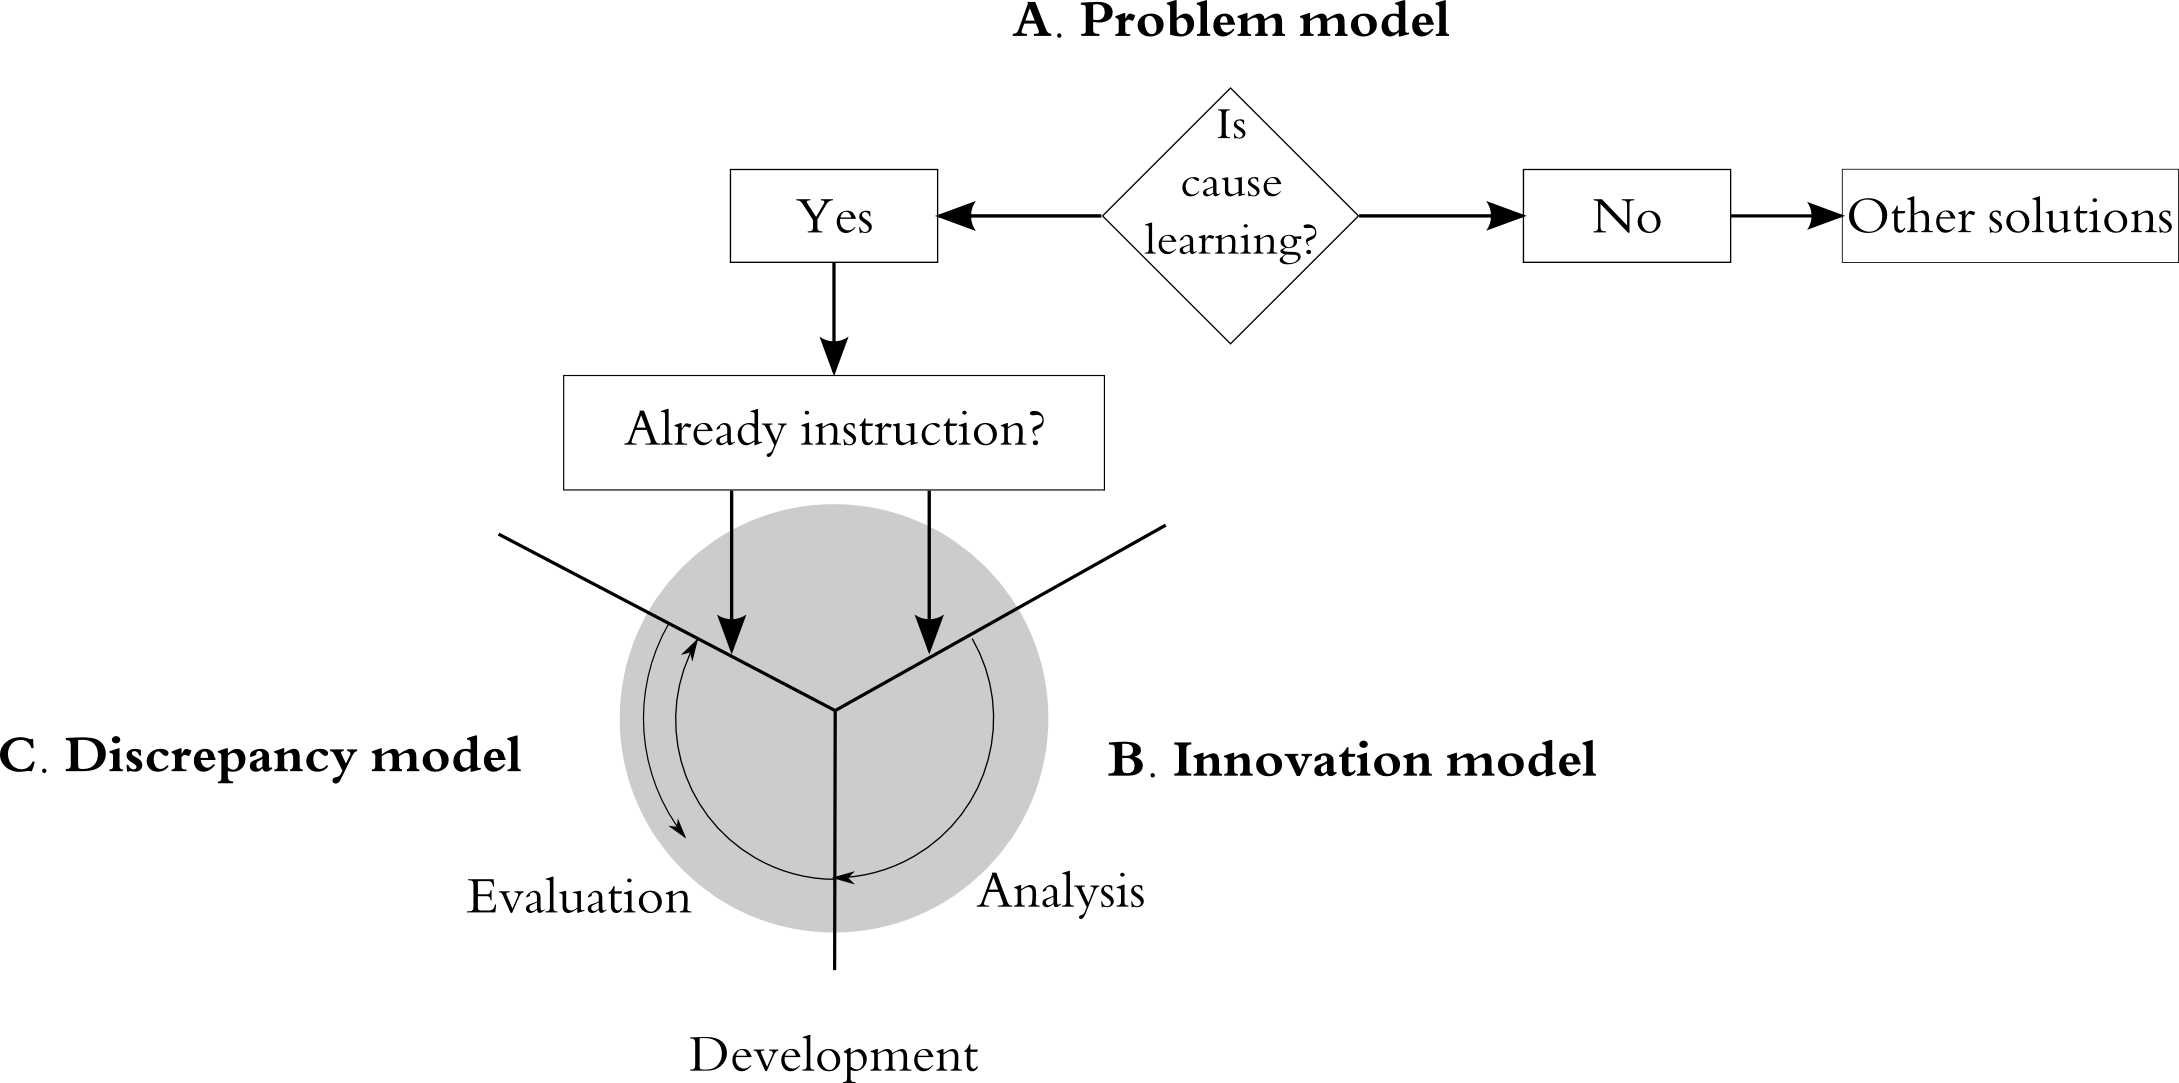
\includegraphics[width=\textwidth]{needsassessment}
\caption{\footnotesize The three sides of needs assessment \protect\cite{smithragan}\label{fig:needsassessment}}
\end{figure}

In the case of the instruction which will be constructed for this assignment, at first the problem model will be used to investigate the problem, and which of the two follow-up models should be used for the needs assessment.

\subsubsection{The problem}

In the Netherlands, quantum mechanics always used to be a topic which schools themselves could choose to teach or not to teach. The only skill students had to know for the Centraal Eindexamen (the national central exams at the end of high school) which comes close to quantum mechanics is to elucidate the photoelectric effect and the wave-particle duality, mentioned within point 20 under subdomain E3 \cite{eindexamen2015}. However, one of the changes in the Centraal Eindexamen of 2016 was the addition of domain F1, which is called Quantum world \cite{eindexamen2016}. For this subdomain the candidate has to be able to apply the wave-particle duality and the uncertainty principle of Heisenberg, and to explain the quantization of energy levels in some examples with a simple quantum physical model. In order to give all candidates a chance of passing this subdomain, schools have to alter their programs in order to meet the expectations of the Centraal Eindexamen.

However, when searching the internet using the search machine Google concerning the implementation of quantum mechanics in Dutch high schools, the quantity and the quality of the results are very low. There are also no results to be found in the Dutch papers. An example is the Dutch site http://www.quantumuniverse.nl/, where teachers can find a small amount of brief courses on fundamental quantum mechanics, and where the forums are very quiet with only 5 discussions, of which 4 are just started threads from the site administrator.

Upon finding this information, an expert was consulted to confirm this conjecture. The expert was researching the implementation of quantum mechanics on middle schools, and she also a first degree physics teacher. She stated that within her school there were no initiatives to bring this topic in their classrooms, and that their school was no exception as well.

The fact that next year domain F1 has to be fully implemented and taught to all vwo students who chose physics as an examination subject is therefore slowly turning into a sword of Damocles. This stresses the urgency for the development of new course material. This is an example of extrinsic motivation. However, is there also intrinsic motivation to teach quantum mechanics on high schools? First of all, there is no article which claimed that quantum mechanics should not be taught on high schools. On the other hand there are but a few authors who did have some arguments in favour of teaching. \citeA{muller} and \citeA{henriksen} state that quantum mechanics shapes our world view and that educated citizens should therefore become acquainted with the topic. It is also regarded as fundamental and should therefore be taught \cite{henriksen,hobson}. Finally, \citeA{erduran} states that the teaching of philosophical themes in science education has been advocated for several decades, and quantum mechanics is one of these themes.

Because it involves new instruction, the innovation model will be used for the second part of this needs assessment.

\subsubsection{The innovation}
\label{sssec:needsassessmentinnovation}

The nature of the innovation lies within the change of the Centraal Eindexamen of 2016 in respect to the Centraal Eindexamen of 2015. The new additions within the domain Kwantumwereld outline the new goals of physics education in the Netherlands, and will be the ultimate goals for the students to achieve, and therefore be the ultimate learning goals for the students to achieve. This results in the following learning goals \cite{eindexamen2016}:

The candidate can:
\begin{itemize}
\item describe quantum phenomena in terms of the enclosure of a particle:
\begin{itemize}
\item estimate whether quantum phenomena are to expected by comparing the debroglie-wavelength with the order of largeness of the enclosure of the particle;
\item apply the uncertainty principle of Heisenberg;
\item describe the quantum model of the hydrogen atom and calculate the possible energies of the hydrogen atom;
\item describe the quantum model of a particle in a one-dimensional energy well and calculate the possible energies of the particle;
\item Bohr radius, zero-point energy.
\end{itemize}
\item describe the quantum-tunnel effect with a simple model and indicate how the chance of tunneling depends on the mass of the particle and the height and width of the energy-barrier,
\begin{itemize}
\item minimal in the contexts of: Scanning Tunneling Microscope, alpha-decay.
\end{itemize} 
\end{itemize}

These goals confirm what the literature describes about the current appliance of quantum mechanics teaching within secondary, namely that often quantum mechanics is introduced with great emphasis on learning and practising algorithmic skills \cite{papaphotis1,papaphotis2}. However, it is also found that high school students show higher interest in the conceptual aspects than the algorithmic aspects \cite{papaphotis1,papaphotis2,levrini}. When focusing on the conceptual aspects, it engages students \cite{henriksen} and students start asking fundamental questions \cite{mckagan}. Furthermore, mathematical oriented approaches might be more common, however, quantum mechanics is regarded to be mathematically challenging \cite{gianino, mckagan}, and most high school students lack proper background in mathematics at the required level \cite{dori}. Because the usual focus on the algorithmic aspects, students often do not learn what instructors want them to learn \cite{asikainen, mckagan}, and improved student learning is possible by shifting the focus to conceptual understanding \cite{mckagan}.

Therefore, the aim of this instruction is to focus on a conceptual approach instead of a mathematical approach. Then, after the students have a sufficiently conceptual understanding of the material, the concurrent instructions in the curriculum can emphasise the goals stated by the Centraal Eindexamen of 2016, which adds the mathematical layer on top of the conceptual layer and can deepen the understanding of quantum mechanics. In summary, the main goal of this instruction is \emph{to provide the student with a conceptual understanding of the different phenomena occurring in the realm of quantum mechanics}.

%learning environment

\subsection{Learning Environment}

The learning environment description is the other major component of the learning context analysis \cite{smithragan}. The description contains information of all the external factors influencing the instruction. These are the mediators of the instruction, the already existing curricula which takes place in the environment, the available equipment available on the location of the instruction, the characteristics of the facilities at the location of the instruction, the characteristics of the organisation in which the instruction will take place, and the philosophies and taboos of the larger community in which this organisation exists.

A current first degree teacher training \cite{leraarnatuurkundemaster} does encompass quantum mechanics, so teachers which had this training should be familiar to the domain. However, \citeA{asikainen} states that teachers often still possess misconceptions about quantum mechanics, which are comparable to the misconceptions of the students themselves. These misconceptions will be discussed in the learner analysis section on page~\pageref{subsec:misconceptions}. Experienced teachers who are teaching modern physics are more capable of teaching quantum mechanics \cite{asikainen}.

When implementing the instruction, the placing within the already existing curriculum is also important, because the instruction depends on prerequisites from other elements of the curriculum. The main prerequisite is knowledge of Bohr his atom model, because the different particles within this model are the particles on which quantum mechanics apply. This knowledge is taught in Domain E from the centraal eindexamen \cite{eindexamen2016}, and because of the prerequisite, it is of upmost importance that this instruction is placed after Domain E in the existing curriculum. As already described in the needs assessment, the conceptual instruction could be followed by instruction of the mathematical aspects of quantum mechanics. Also, various experiments could be taught, which demonstrate the discovery of the various concepts introduced in the instruction and explain the different principles between the concepts. This could for example be the EPR experiment \cite{kuttner, muller, velentzas}, which could lead to critical assessment of the realist and ontologist perceptions on quantum mechanics.

Another important aspect of the instructional environment is the method of delivery \cite{smithragan}. The recommendations for different aspects of the medium used for the delivery of the instruction entail interactivity, visualisation, the combination of different modes of representation, and the use of computation. By making it able to interact with the medium, it is possible for students to experiment with the different concepts, which gives way to inquiry learning \cite{adegoke, asikainen, dori, mckagan}. Visualisation is a powerful tool, and can make the matter less abstract \cite{dori, henriksen, mckagan}. It also is easier to build mental models of quantum mechanics. \citeA{levrini} warns however against the use of oversimplified visualisations, because pictures are extremely partial and can be misleading. Therefore, it is important that the visualisation does not entail any unnecessary simplified representation of the matter. This combined with other different modes of representation, for example a textual description of the concept, makes it possible for the student to complete their mental model \cite{dori}. Finally, the use of computation makes it possible to take away the mathematical complexity from quantum mechanics, making way for a purely conceptual approach \cite{barnes, mckagan, velentzas}.

One could combine all these aspects by using simulations, which is also recommended by \citeA{mckagan}. However, teachers often prefer traditional lectures, because that is easier to implement in their classroom \cite{adegoke}. This difficulty has to be overcome if quantum mechanics is to be implemented successfully in the classroom. Furthermore, it has to be investigated whether the sufficient hardware is available in the learning environment.

Finally, it is important to investigate whether the instruction fits in with the mission and vision of the school, and also the philosophies and taboos that the teachers hold. Therefore, it is advised to find these discrepancies by the means of interviews, in which the school board is asked about their mission and vision, and the teachers about their personal believes in regard to quantum mechanics.

In any case, this assignment does not look into the implementation of the instruction yet, so these factors have to be looked closer at when embedding the instruction in the context of a specific school.

% Learner analysis

\section{Learner Analysis}
\label{sec:misconceptions}

The second analysis is that of the learners \cite{smithragan}. The purpose of this analysis is the characterisation of the end user of the instruction, which is in this case the students of secondary education in the Netherlands, mostly ranging from age 17 to 18. This analysis will focus itself on the general misconceptions held by members of this demographic.

When developing an instruction, it is important to consider the already available conceptions on the topic. In quantum mechanics, these preconceived models often prove to be incorrect \cite{asikainen, papaphotis2, thacker}. This partly comes from the nature of quantum theory \cite{papaphotis2}, but also partly from textbooks and instruction \cite{hubber, papaphotis2}. The problems often stem from depending on outdated deterministic or realist models \cite{hubber, papaphotis1, papaphotis2}, an often mentioned example of this is that students often mix up the deterministic planetary model with the indeterministic atom model \cite{dori, henriksen, hubber, muller, papaphotis1, papaphotis2}. \citeA{mckagan} also mentions that it is difficult for students to recognise the scale in which quantum mechanics take place.

\citeA{thacker} describes how much knowledge of students consists out of memorised facts, for example that light is a wave and electrons are particles. When the student then is confronted with new or different information from what they know, they develop new memorised facts instead of creating the right model. This then results in models consistent with fragmented models of microscopic processes, which are often incorrect but self-consistent with a certain experiment \cite{hubber, thacker}. When the student cannot model the fragments anymore, this can result in deep skepticism towards quantum mechanics \cite{barnes, henriksen, levrini}. \citeA{muller} has created a long list of exact conceptions students hold about microscopic phenomena, which are too detailed to enlist fully in this article.

% Task analysis

\section{Task Analysis}

The final step is analysing the learning task \cite{smithragan}. In this analysis the goals from the needs assessment during the analysis of the learning context have to be translated to test specifications, with which the content of the instruction can be established. In order to achieve these test specifications, first the type of learning has to be established. Having this established, a information-processing analysis corresponding to the type of learning can be conducted \cite{smithragan}. \citeA{dance} provides a clear conceptual understanding of quantum teleportation, and will therefore be used to conduct this information-processing analysis. The next step is the prerequisite analysis. The outcome of this has to correspond to the outcome of the learner analysis. Finally, the learning objectives can be written, which form the test specifications. Every learning objective has to contain a description of the terminal behaviour or actions that will demonstrate learning, a description of the conditions of demonstration of that action and a description of the standard or criterion \cite{smithragan}. Every learning objective will fall into a category of Bloom his taxonomy of learning objectives \cite{bloom}, and will use appropriate action verbs. Most learning objectives within will be knowledge objectives, because there is a lot of new knowledge which has to be provided and it forms the basis for all other objectives. There will be no or very few synthesis and evaluation objectives, because these objectives would take too much time within the instruction to achieve to be feasible to use.

\subsection{Learning goal}

The main learning goal as specified needs assessment using the innovation model from page~\pageref{sssec:needsassessmentinnovation}, the instruction will pursue provide the student with a conceptual understanding of the different phenomena occurring in the realm of quantum mechanics. This goal will be the main guideline for the information-processing analysis. However, it will not be possible to provide the students with a complete conceptual understanding of quantum mechanics. First of all, not even the scientific community has a full grasp of quantum mechanics, because it is a relatively new and still developing subject area. Second to that, physics students in secondary education do not have the time needed to gain at least the complete conceptual understanding of quantum mechanics available from the scientific community. Finally, there is not enough time to design an instruction which achieves a complete conceptual understanding, and the time available for this instruction is also limited. Therefore a choice has to be made in the different topics being taught.

Furthermore, there exists a consensus within the studied articles that quantum mechanics is a difficult topic, and this is also a consensus among educators \cite{gianino,papaphotis1,papaphotis2}. There are a couple of reasons mentioned within the articles to explain this topical difficulty. A couple of sources state that quantum mechanics is a very counter intuitive topic \cite{henriksen, levrini, mckagan, singh2}, because it contradicts many aspects of our daily experience, like locality or determinism. Quantum mechanics is also considered to be a very abstract topic \cite{barnes, gianino, mckagan, papaphotis1, singh1}. Because quantum mechanics differs a lot from our everyday experiences and because of its abstractness, it is difficult for learners to visualise the concepts of quantum mechanics \cite{henriksen, mckagan}. Another factor contributing to the difficulty of quantum mechanics is that it is mathematically challenging \cite{gianino, mckagan}, it involves mathematical skills that most high school students --- even vwo 6 students --- do not possess. Because of the difficulties stemming from teaching quantum mechanics, it would be better to teach concentrate on teaching a few topics of quantum mechanics in a way that it can be understood, rather than trying to teach as much as possible in the limited time available.

\subsection{Types of learning}

The literature provides a lot of strategies which can be used to teach quantum mechanics. There are recommendations for which content to use. Some of the strategies focus on meta-cognitive aspects. Finally, there are a few frameworks which can be used to teach modern physics.

Some of the content-related strategies emphasise the importance of embedding the instruction in real-world contexts, for they help with understanding \cite{mckagan,thacker,dori} and help appreciate the relevance of quantum mechanics \cite{barnes, henriksen, mckagan}. Furthermore, \citeA{thacker} suggests introducing microscopic processes as an integral part of a study of electricity and magnetism. This could help demystify the topic, which also would contribute towards a better understanding \cite{barnes, muller}. An example of how this can be done is by using the e/m experiment, where the electromagnetic effect is demonstrated by the properties of electrons. Furthermore, the language of physics is important \cite{henriksen}, and should be used carefully \cite{mckagan}. The consulted articles all recommend a conceptual approach above a mathematical-oriented approach. Mathematical-oriented approaches might be more common, but most high school students lack proper background in mathematics at the required level \cite{dori}. \citeA{barnes} and \citeA{henriksen} believe teaching through history of science is believed to be constructive.

\citeA{papaphotis1} states that critical thinking skills are crucial for understanding quantum mechanics, because students have to investigate the new material in a critical way to build the correct mental models. Active learning also contributes to investigation of the material. Because the students easily build misconception, right feedback is vital to prevent misconceptions and can stimulate students to build correct mental models. Finally, \citeA{papaphotis1} suggests collaboration, which is also suggested by \citeA{adegoke} and \citeA{barnes}. Collaboration could lead to peers providing each other with critical questions and feedback. Especially in the case of female students this could benefit to learning quantum mechanics \cite{adegoke}. 

The frameworks mentioned by different authors are directly or very similar to thought experiments \cite{asikainen, erduran, levrini, velentzas}. Asikainen describes the most elaborated framework for a well-conducted thought experiment, which includes the steps question and general assumptions, description of the features of the system, performance of the thought experiment itself, extraction of the results and drawing conclusions. \citeA{erduran} and \citeA{levrini} also describe a framework, but the steps they mention already overlap with those of \citeA{asikainen}.

\subsection{Information-processing analysis}

\subsection{Prerequisite analysis}

Furthermore, it is important to look at the pre-existing knowledge about quantum mechanics of the students. According to the Centraal Eindexamen 2016 \cite{eindexamen2016}, the candidate should already have learned the Rutherford-Bohr Model of the Atom, and this is earlier already specified as prerequisite of the instruction. This means that the students have knowledge of at least two elementary particles, namely the photon and the electron, and their place within the atom. They also should know about the nucleus and the shell of an atom, and about protons and neutrons. Furthermore, it could be that the students already learned about the double-slit experiment \cite{eindexamen2015}, although it would be better if the students get instruction about this experiment after this instruction. This is because then they will be familiar with terms like superposition and observer dependency, which are necessary to fully comprehend the double-slit experiment. Finally, the students could have learned about some of the concepts of quantum mechanics outside of the standard curriculum, like for example via science magazines. However, for this instruction it will be presumed that they have no knowledge of these concepts, for the reason that they have not been taught in the standard curriculum.

\subsection{Learning objectives}

\subsection{Test specifications}

%%% DESIGN

\chapter{Design}
\thispagestyle{fancy}

%%% DEVELOPMENT

\chapter{Development}
\thispagestyle{fancy}

%%% FORMATIVE EVALUATION

\chapter{Formative Evaluation}
\thispagestyle{fancy}

\bibliographystyle{apacite}
\bibliography{references}

\end{document}
